\documentclass[oneside,12pt]{report}
\usepackage[a4paper,top=2cm,right=2cm,bottom=2cm,left=2cm]{geometry}
\usepackage[utf8]{inputenc}
\usepackage[utf8]{vietnam}
\usepackage{multirow}
\usepackage{tikz}
\usetikzlibrary{calc}
\usepackage{fancyhdr}
\usepackage{xcolor}
\usepackage{titlesec}
\usepackage{chngcntr}
\usepackage{subcaption}
\usepackage{booktabs}
\usepackage{xurl}
\usepackage{indentfirst}
\usepackage{hyperref}
\usepackage{graphicx}
\usepackage{placeins}
\usepackage{enumitem}

\setlength{\headheight}{17.64015pt}
\renewcommand{\familydefault}{\sfdefault}

\pagestyle{fancy}
\setlength{\headheight}{16pt}
\lhead{}
\rhead{\leftmark}
\lfoot{}
\cfoot{\thepage}
\rfoot{}

\titleformat{\chapter}[display]{\flushright\bf\huge\color{red}}{\chaptertitlename\ \thechapter}{10pt}{}
\titleformat{\section}{\bf\Large\color{red}}{\thesection}{10pt}{}
\titleformat{\subsection}{\bf\large\color{red}}{\thesubsection}{10pt}{}
\titleformat{\subsubsection}{\bf\normalsize\color{red}}{\thesubsubsection}{10pt}{}

\newcommand{\jmeter}{\textbf{Apache JMeter}}
\newcommand{\apache}{\textbf{Apache}}
\newcommand{\java}{\textbf{Java}}

\begin{document}

\begin{titlepage}
    \begin{tikzpicture}[remember picture, overlay]
        \draw[double,double distance=5pt,ultra thick] ($(current page.north west) + (2cm,-2cm)$) rectangle ($(current page.south east) + (-2cm,2cm)$);
    \end{tikzpicture}

    \begin{center}
        \vfill
        {\LARGE\bf Kiểm thử và đảm bảo chất lượng phần mềm} \\
        {\Large\bf INT3117 1, học kỳ II năm học 2020$-$2021} \\
        \bigskip
        \bigskip

        \bigskip
        {\Huge\bf Tìm hiểu công cụ Apache Jmeter}
        \bigskip

        \bigskip
        \bigskip

        % chktex-file 44
        \begin{tabular}{c|l}
            \multirow{2}{*}{Thành viên nhóm} & Ngô Quang Dương (17020191) \\
            & Nguyễn Phương Hiếu (17020747) \\
        \end{tabular} \\
        \medskip
        {\today}
        \vfill
    \end{center}
\end{titlepage}

\tableofcontents

\chapter{Giới thiệu}

\section{Lịch sử}

\par \jmeter{} là một dự án mã nguồn mở của \apache{}, được viết hoàn toàn bằng \java{}. Mã nguồn của dự án được public trên GitHub:~\url{https://github.com/apache/jmeter}

\par Người đầu tiên phát triển \jmeter{} là \href{https://www.linkedin.com/in/stefanom}{Stefano Mazzocchi}. Ban đầu, anh tạo ra công cụ này để kiểm tra hiệu năng cho một dự án web server là \textbf{Apache JServ}, dự án mà sau này được thay thế bằng \textbf{Apache Tomcat}. Phiên bản 1.0 của \jmeter{} được đưa ra vào cuối năm 1998. Từ đó đến nay, các tính năng của \jmeter{} liên tục được bổ sung và nâng cao.

\par Ban đầu, \jmeter{} chỉ được thiết kế để kiểm tra hiệu năng của các ứng dụng web. Về sau, \jmeter{} được cung cấp thêm các tính năng khác cho việc kiểm thử chức năng và hiệu năng.

\section{Cài đặt}

\par Ở thời điểm báo cáo này được viết, phiên bản mới nhất của \jmeter{} là 5.4.1. \jmeter{} có thể được tải về dưới một trong hai dạng: \textit{mã nguồn} và \textit{binaries} từ website
\begin{quotation}
  \url{https://jmeter.apache.org/download_jmeter.cgi}
\end{quotation}

\par Phiên bản này yêu cầu máy có \java{} 8+. Nếu chọn cách tải mã nguồn, máy cần được cài thêm Gradle để biên dịch.
\bigskip
\par Các phiên bản trước của \jmeter{} có thể được tải về từ link lưu trữ
\begin{quotation}
  \url{https://archive.apache.org/dist/jmeter/binaries/}
\end{quotation}

\bigskip
\par Đối với lựa chọn tải binaries, sau khi tải về và giải nén, ta có được một cấu trúc thư mục như sau:

\begin{verbatim}
bin/
  - examples/
  - report-template/
  - templates/
docs/
  - api/
  - css/
  - images/
extras/
lib/
  - ext/
  - junit/
licenses/
printable_docs/
  - demos/
  - extending/
  - localising/
  - usermanual/
\end{verbatim}

\par Trong các thư mục trên, cần lưu ý nhất tới \texttt{bin/} và \texttt{lib/}.

\begin{itemize}[itemsep=0pt]
  \item \texttt{bin/} chứa các file thực thi để sử dụng \jmeter{}.
  \item \texttt{lib/} chứa các file JAR $-$ là các plugins, các extensions cho \jmeter{}.
\end{itemize}

\par Để bắt đầu sử dụng \jmeter{}, truy cập thư mục \texttt{bin/} (từ Powershell/Command Prompt nếu sử dụng Windows, từ Terminal nếu sử dụng Linux/Mac), sau đó
\begin{itemize}[itemsep=0pt]
  \item Chạy file \texttt{jmeter.bat} nếu máy sử dụng Windows.
  \item Ngược lại, chạy file \texttt{jmeter}.
\end{itemize}

\par Sau đó, giao diện đồ họa của \jmeter{} hiện lên như sau:

\FloatBarrier{}
\begin{figure}[htp]
  \centering
  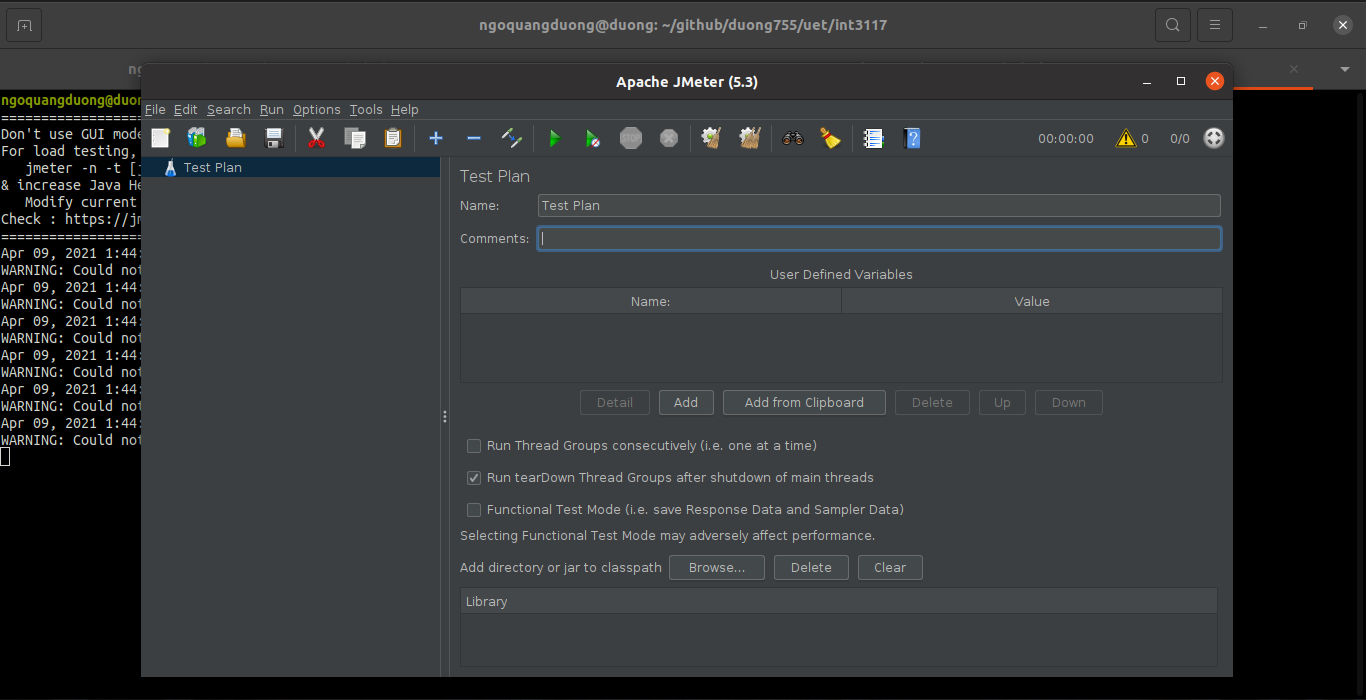
\includegraphics[scale=0.33]{jmeter-gui.png}
  \caption{Giao diện đồ họa của \jmeter{}}
\end{figure}
\FloatBarrier{}

\par Có thể có lỗi khi chạy \jmeter{} trên Linux, như việc không tìm thấy một class, chẳng hạn
\begin{quotation}
\texttt{org.GNOME.Accessibility.AtkWrapper}
\end{quotation}

\par Để khắc phục điều này, hãy comment lại các class trong file
\begin{quotation}
\texttt{/etc/java-8-openjdk/accessibility.properties}
\end{quotation}
\par và khởi động \jmeter{} một lần nữa.

\chapter{Một số tính năng}

\section{Kiểm tra hiệu năng}

\section{Test IDE}

\section{Tạo báo cáo}

\section{Khả năng mở rộng}

\section{Khả năng tích hợp với các công cụ khác}

\chapter{So sánh}

\section{Selenium IDE}

\section{Gatling}

\end{document}
